%%%%%%%%%%%%%%%%%%%%%%%%%%%%%%%%%%%%%%%%%%%%%%%%%%%%%%%%%%%%%%%%%%%%%%%%%%%
%% This file is part of the book
%%
%% Algorithmic Graph Theory
%% http://code.google.com/p/graph-theory-algorithms-book/
%%
%% Copyright (C) 2009, 2010, 2011 Minh Van Nguyen <nguyenminh2@gmail.com>
%%
%% See the file COPYING for copying conditions.
%%%%%%%%%%%%%%%%%%%%%%%%%%%%%%%%%%%%%%%%%%%%%%%%%%%%%%%%%%%%%%%%%%%%%%%%%%%

\documentclass{article}

\usepackage{subfigure}
\usepackage{tikz}
\usetikzlibrary{external}
\tikzexternalize{distinct-trees-specified-order-4}

\begin{document}

\begin{figure}
\subfigure[]{
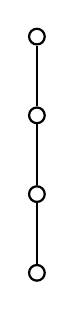
\begin{tikzpicture}
[nodeDecorate/.style={shape=circle,inner sep=2pt,draw,thick},%
  lineDecorate/.style={-,thick}]
%% nodes or vertices
\foreach \nodename/\x/\y in {1/0/0, 2/0/1, 3/0/2, 4/0/3} {
  \node (\nodename) at (\x,\y) [nodeDecorate] {};
}
%% edges or lines
\path
\foreach \startnode/\endnode in {1/2, 2/3, 3/4} {
  (\startnode) edge[lineDecorate] node {} (\endnode)
};
\end{tikzpicture}
}
\quad
%%
%%
\subfigure[]{
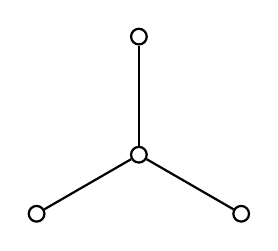
\begin{tikzpicture}
[nodeDecorate/.style={shape=circle,inner sep=2pt,draw,thick},%
  lineDecorate/.style={-,thick},
  scale=1.5]
%% nodes or vertices
\foreach \nodename/\x/\y in {1/-0.8660/-0.5, 2/0.8660/-0.5, 3/0/1, 4/0/0} {
  \node (\nodename) at (\x,\y) [nodeDecorate] {};
}
%% edges or lines
\path
\foreach \startnode/\endnode in {1/4, 2/4, 3/4} {
  (\startnode) edge[lineDecorate] node {} (\endnode)
};
\end{tikzpicture}
}
\end{figure}

\end{document}
